\let\conjugatet\overline
\section{Implementierung des Empfängers}
\label{sec:impl_des_receivers}
Bei der Übertragung treten Störungen und Effekte auf, die das Empfangssignal vom Sendesignal abweichen lassen. Vor der Demodulation und Auswertung der Daten ist die erste Stufe des Empfängers deshalb eine Synchronisation. Ziel der Synchronisation ist das Empfangssignal so zu korrigieren, dass es dem Sendesignal wieder möglichst nahe kommt. Die anschließende Kanaldecodierung und Auswertung der Daten im FIC und MSC findet in den entsprechenden hierarchischen GNU Radio Blöcken statt. Abb.~\ref{fig:grc_receiver} zeigt den Aufbau eines DAB+ Empfängers im GRC.

\begin{figure}[h]
\centering
  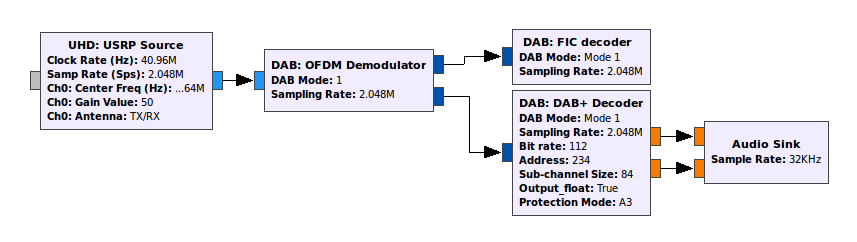
\includegraphics[width=\textwidth]{figures/GRC_receiver.png}
	\caption{DAB+ Empfänger im GRC}
	\label{fig:grc_receiver}
\end{figure}

Das Empfangssignal $R(t)$ wird in folgender Beziehung zum Sendesignal $S(t)$ angenommen:
\begin{equation}
R(t) = a(t,f) \cdot S(t-\tau_{off}) \cdot e^{j(2 \pi f_{off} t + \varphi_{off})} + N(t)
\end{equation}
Das Signal wird um einen Zeitoffset $\tau_{off}$ verzögert und hat wegen Doppler-Verschiebungen und Ungenauigkeiten der Oszillatoren einen Frequenzoffset $f_{off}$. Ein konstanter Phasenoffset $\varphi_{off}$, der durch Reflektionen der Welle entsteht, wirkt sich in diesem Fall nicht auf das demodulierte QPSK Signal aus, da sich wegen der differentiellen Modulation eine konstante Phase bei der Differenzbildung heraushebt. Es ist also keine Kanalschätzung nötig. Die Amplitude des Signals wird durch frequenzselektives Fading über der Zeit und der Frequenz unterschiedlich stark gedämpft. Wegen der Schmalbandigkeit der einzelnen Unterträger bei OFDM kann der Kanal trotzdem in jedem Unterträger als flach angenommen werden, woraus $a(t,f)=a(t)$ folgt. Die Dämpfung des Signals ist für die Symbolentscheidung bei PSK zudem nicht ausschlaggebend. Letztendlich wird das Signal noch durch \ac{AWGN} überlagert.\\ 
Um eine möglichst optimale Synchronisations zu erreichen, werden in der folgenden Signalverarbeitungskette relevanten Effekte schrittweise gemessen und korrigiert.

\subsection{Zeit Synchronisation}
\label{sec:time_sync}
Eine geeignete Zeitsynchonisation muss sowohl eine grobe Synchronisation des OFDM Frames, als auch eine feine Synchonisation der einzelnen OFDM Symbole sicherstellen. \\
Der Beginn jedes Frames $ k $ wird durch das Nullsymbol $z_{0,k}$ markiert. Wegen $S(t) = 0$ für $t \in [0, T_{NULL}]$ stellt es eine zuverlässige Möglichkeit dar, den Anfang von Frames über eine Energiemessung zu detektieren. Die Energiemessung lässt sich über eine Autokorrelation des Signals realisieren.

\begin{equation}
E[i] = \sum \limits_{j=i}^{T_G}|x[j]|^2
\label{eq:energy}
\end{equation}

Nachdem der Anfang eines Frames detektiert wurde, muss im Folgenden der Beginn jedes OFDM Symbols $z_{l,k}$ ($l \in [1, 76]$) festgelegt werden. Diese feine Zeitsynchronisation erfordert keine sehr hohe Genauigkeit, da jedem Symbol ein \ac{CP} der Dauer $T_G = 246$ \textmu s vorgeschoben ist, dessen Inhalt dem Ende des eigentlichen Symbols entspricht. Dadurch ergibt sich ein Zeitbereich von  $T_D \in [0,T_G]$, in dem der Symbolanfang fehlerfrei gesetzt werden kann. Das gesetzte Symbolfenster kann also nicht in das vorhergehende oder nachfolgende Symbol hineinragen.

\begin{figure}[htb]
\centering
  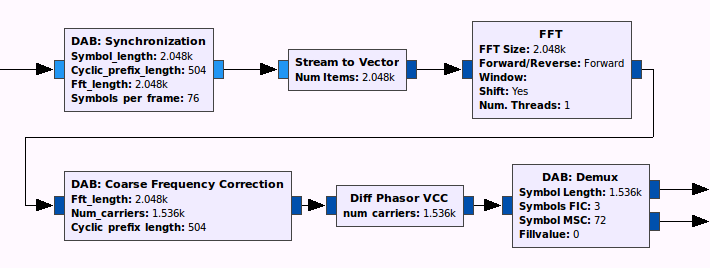
\includegraphics[width=0.9\textwidth]{figures/sync_hier_block.png}
	\caption{Aufbau der kompletten Synchronisationskette im \ac{GRC}}
	\label{fig:sync_overview}
\end{figure}

Um \ac{ISI} zu minimieren ist der theoretisch optimale Abtastzeitpunkt genau am Ende des CPs zu wählen. Eine komplette \ac{ISI} Unterdrückung ist wegen $T_G < \tau_{max}$ mit einer maximalen Echo Verzögerung von $\tau_{max} = 300$ \textmu s nicht möglich \cite{dab_buch}. Jedoch wird die \ac{ISI} zu einem Minimum reduziert, wenn ein maximal später Startpunkt gewählt wird, da die Interferenzzeit $\tau_{max} - T_D$, bei $\tau_{max} < T_G+T_S$, dadurch minimiert wird.\\

Um den exakten Anfang eines Symbols zu bestimmen, wird die zyklische Wiederholung des Symbolanteils im \ac{CP} genutzt. Durch eine Korrelation des abgetasteten Empfangssignals $r[i]$ mit einer um $T_S$ verzögerten Version desselben Signals $r[i+T_S]$ über das Intervall $[i, i+T_G]$ kann der Anfang des \ac{CP} über einen Peak der Korrelation identifiziert werden.

% cyclic prefix figure
\begin{figure}[h]
\begin{center}
\begin{tikzpicture}
\newcommand{\ursprung}{(0,0)}
\node[] at \ursprung (null) {}; 
\draw [thick, rounded corners = 6pt] 
    (null) -- ++(0,0.5) -- ++(0,0.5) -- ++(8,0) -- ++(0,-1) -- ++(-8,0) -- ++(0,0.5);
\draw [dashed]
    (null)+(2,0) -- ++(2,1);
\draw [dashed]
    (null)+(6,0) -- ++(6,1);
\node[] at (1,1.5) (guard) {$T_G$};
\draw [<-] (0,1.5) -- (guard.west);
\draw [->] (guard.east) -- (2,1.5);
\node[] at (5,1.5) (symbol) {$T_S$};
\draw [<-] (symbol)+(-3,0) -- (symbol.west);
\draw [->] (symbol) -- (8,1.5);
\node[] at (0.75,-0.5) (delay) {$T_D$};
\draw [<-] (delay)+(-0.75,0) -- (delay.west);
\draw [->] (delay) -- (1.5,-0.5);
%Beschriftung
\node[] at (1,0.5) (cp) {CP};
\node[] at (7,0.5) (cp) {CP Quelle};
%Vorgängersymbol
\draw [thick, rounded corners = 6pt]
    (-1.5,0) -- ++(1.5,0) -- ++(0,1) -- ++(-1, 0);
\draw [decorate,decoration={snake, amplitude=.4mm}] (-1.5,0) -- (-1,1);
%Nachfolgersymbol
\draw [thick, rounded corners = 6pt]
    (9,0) -- ++(-1,0) -- ++(0,1) -- ++(1.5, 0);
\draw [decorate,decoration={snake, amplitude=.4mm}] (9,0) -- ++(0.5,1);
%gesetztes Symbolfenster
\draw[-,decorate,decoration=brace] 
    (7.5,-0.2) -- (1.5,-0.2) node [midway, yshift=-0.3cm]{};
\node[] at (4.5,-0.6) {gesetztes Symbolfenster für $z_{l,k}$};
\end{tikzpicture}
\end{center}
\caption{OFDM Symbol und Cyclic Prefix}
\label{chart:cp}
\end{figure}

%einfache correlation
\begin{equation}
y[i] = \sum \limits_{j=i}^{T_G}r[j] \conjugatet{r[j+T_S]}, \ \ y[i] \in \mathbb{C}
\label{eq:corr_einfach}
\end{equation}

Unter Berücksichtigung von AWGN ist r[i]=x[i]+n[i] mit $n[i] \sim \mathcal{N}(\mu,\,\sigma^{2})$ resultiert für die Korrelation

\begin{equation}
    \begin{aligned}
y[i] &= \sum \limits_{j=i}^{T_G}(r[j]+n[j]) \conjugatet{(r[j+T_S]+n[j])} \\
&= \sum \limits_{j=i}^{T_G}x[j] \conjugatet{r[j+T_S]} + \sum \limits_{j=i}^{T_G}r[j] \conjugatet{n[j+T_S]} + \sum \limits_{j=i}^{T_G}n[j] \conjugatet{x[j+T_S]} + \sum \limits_{j=i}^{T_G}n[j] \conjugatet{n[j+T_S]} \\
&= P T_G + 2(P \sigma^2) + \sigma^4 \approx P T_G + 2(P \sigma^2)
    \end{aligned}
\end{equation}

und damit ein SNR des Korrelationssignals von
\begin{equation}
SNR = \frac{P_s}{P_n} = \frac{P T_G}{2 P \sigma^2} = \frac{T_G}{2 \sigma^2}
\end{equation}

Durch eine Mittelung über $T_G = 504$ Samples ist das SNR somit ausreichend groß um eine entprechend genaue Peakdetektion durchführen zu können.

Die Korrelation ist dabei auf die Energieanteile des Cyclic Prefixes und dessen Quelle nach $T_S$ normiert, sodass das Ergebnis unabhängig von der Empfangsleisung bleibt, die durch Empfangsqualität und verwendeter Hardware stark variieren kann.

\begin{equation}
    y_{norm}[i] = \frac{\sum \limits_{j=i}^{T_G}r[j] \conjugatet{r[j+T_S]}}{\sqrt{\sum \limits_{j=i}^{T_G}|r[j]|^2 \sum \limits_{j=i}^{T_G}|r[j+T_S]|^2}} = \frac{\sum \limits_{j=i}^{T_G}r[j]     \conjugatet{r[j+T_S]}}{\sqrt{E[i]E[i+T_S]}}
    \label{eq:norm_corr}
\end{equation}

In Abbildung~\ref{fig:corr} ist die normierte Korrelation aus Gl.~\ref{eq:norm_corr} auf das Empfangssignal berechnet worden. Im Bereich von 2,8 bis 3,0 ms ist im Empfangssignal das Nullsymbol zu erkennen. Ein Peak der Korrelation befindet sich zum Beispiel genau bei 3ms, was dem Ende des Nullsymbols bzw. dem Anfang des Phasenreferenzsymbols entspricht. Es ist zu erkennen, dass die Flanken der Korrelation linear ansteigen. Die Breite einer Flanke entspricht $T_G$, also gerade dem Entscheidungsbereich für $T_D$. Durch die Linearität der Flanke und der Normierung, kann der relative Abtastzeitpunkt innerhalb des CPs über einen Schwellwert eingestellt werden. Der tatsächliche Abtastzeitpunkt wird anschließend mit einer Verzögerung von $T_G$ gesetzt. In der Implementierung von Abbildung~\ref{fig:corr} wurde ein Schwellwert von $0,85$ eingestellt, der sich als guter Kompromiss zwischen \ac{ISI} Unterdrückung und einem Sicherheitsabstand zu $T_D > T_G$ herausgestellt hat. Man beachte, dass bei $T_D > T_G$, Samples vom nachfolgenden Symbol im gesetzen Symbolfenster lägen, was zum Empfang von falscher Information führen würde. Dieser Fall entspricht einer fehlerhaften Zeitsynchronisation.

\begin{figure}[h]
\centering
  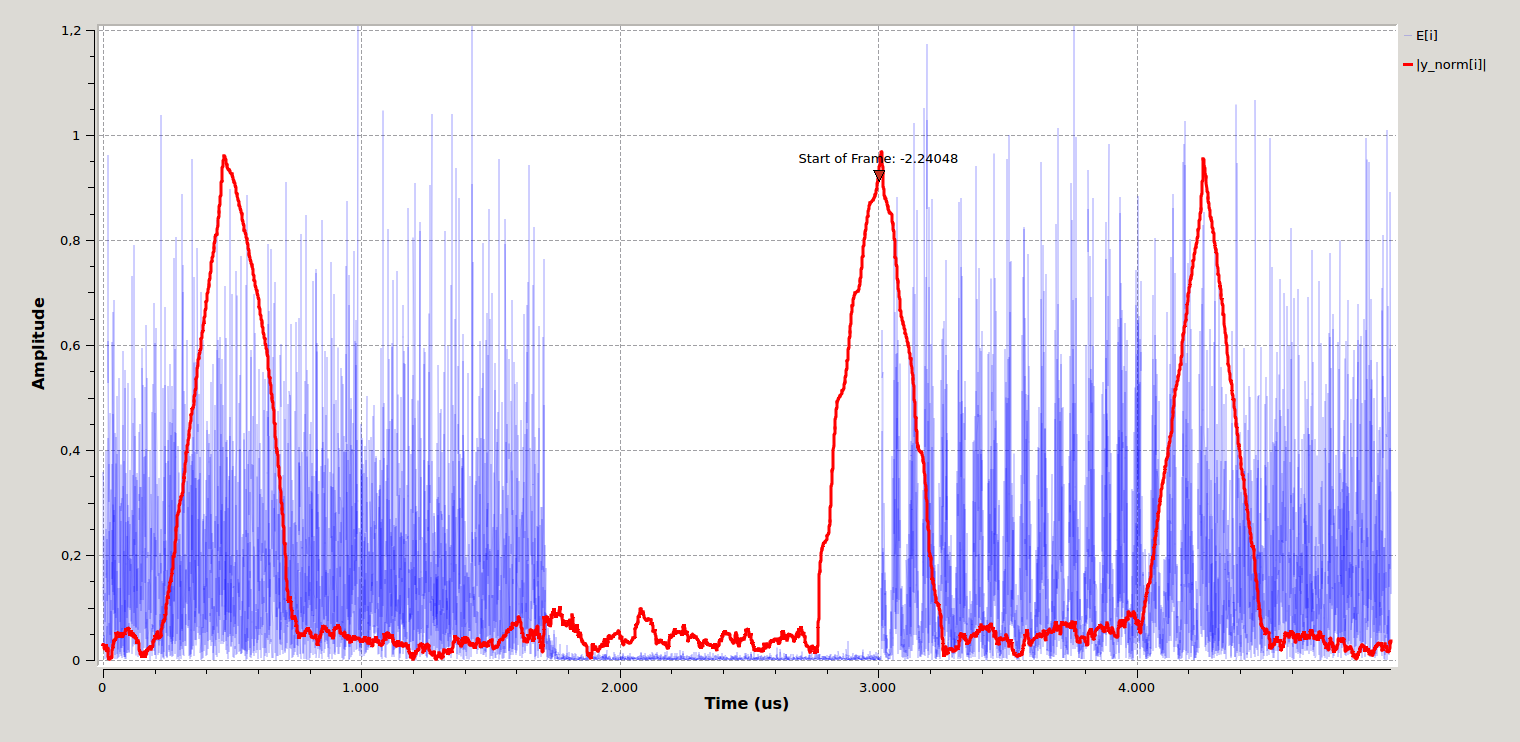
\includegraphics[width=0.8\textwidth]{figures/delayed_correlation_abs_and_energy.png}
	\caption{Korrelation des Cyclic Prefix}
	\label{fig:corr}
\end{figure}

\subsubsection{Implementierung}
Um eine mehrfache Berechnung von Gleichung~\ref{eq:energy} für die Energiemessung, sowie die normierte Korrelation (Gl.~\ref{eq:norm_corr}) zu vermeiden, wurde die feine und grobe Zeitsynchronisation in einer gemeinsamen Klasse implementiert.

\begin{figure}
\begin{center}
\begin{tikzpicture}[node distance = 2cm, auto]
% Define block styles
\tikzstyle{decision} = [diamond, draw, fill=cyan!30, 
    text width=4.5em, text badly centered, node distance=3cm, inner sep=0pt]
\tikzstyle{start} = [rectangle, draw, fill=cyan!30, 
    text width=5em, text centered, rounded corners, minimum height=4em]
\tikzstyle{output} = [trapezium, draw, fill=cyan!30, 
    text width=4em, text centered, minimum height=4em, trapezium right angle=110, trapezium left angle=70]
\tikzstyle{block} = [rectangle, draw, fill=cyan!30, 
    text width=5em, text centered, minimum height=4em]
\tikzstyle{line} = [draw, -latex']
\tikzstyle{cloud} = [draw, ellipse,fill=red!20, node distance=3cm,
    minimum height=2em]
    % Place nodes
    \node [start] (init) {Start};
    \node [decision, below of=init] (null) {NULL erwartet?};
    \node [block, below of=null, node distance=3cm] (corr) {gleitende Korrelation};
    \node [decision, below of=corr, node distance=3cm] (peak) {Peak?};
    \node [block, below of=peak, node distance=2.5cm] (energy) {Energie- messung};
    \node [decision, below of=energy] (first) {Symbol $z_{1,k}$?};
    \node [output, below of=first, node distance=3cm] (tag) {Start des Frames in $T_G$};
    \node [block, right of=null, node distance=4.5cm] (skip) {überspringe $T_S$};
    \node [block, below of=skip, node distance=3cm] (corr2) {einmalige Korrelation};
    \node [decision, below of=corr2] (peak?2) {Peak?};
    \node [above of=null, node distance=2cm] (backtonull){};
    \node [output, below of=peak?2, node distance=3cm] (lost track){nicht mehr in Sync};
    
    \path [line] (init) -- (null);
    \path [line] (null) -- node {ja} (corr);
    \path [line] (null) -- node {nein} (skip);
    \path [line] (corr) -- (peak);
    \path [line] (peak) -- node {ja} (energy);
    \path [line] (energy) -- (first);
    \path [line] (first) -- node {ja} (tag);
    \path [line] (peak) -- node {nein} ++(2.5cm,0);
    \path [line] (first) -- node {nein} ++(2.5cm,0) |- (corr);
    \path [line] (skip) -- (corr2);
    \path [line] (corr2) -- (peak?2);
    \path [line] (peak?2.south) -- node {nein} (lost track);
    \path [line] (peak?2.east) -- node{ja}++(1cm,0) -- ++(0,8cm) -- ++(-6.5,0);
    \path [line] (tag) -- node{}++(0,-1cm) -- node {} ++(-2.5cm,0) -- node{}++(0,17.5cm) -- ++(2.5cm,0);
    \path [line] (lost track.south) -- ++(0,-1cm) -- ++(-2,0);
\end{tikzpicture}
\end{center}
\caption{Programmablaufplan der Zeitsynchronisation}
\label{chart:zeitsync}
\end{figure}

Abbildung~\ref{chart:zeitsync} zeigt den Programmablaufplan der Zeitsynchronisation. Er ist aufgeteilt in die beiden Zweige \glqq Suche Frame Start\grqq{} und \glqq Kontrolle\grqq{}. Der Zweig \glqq Suche Frame Start\grqq{} kommt bei einem der folgenden Fälle zum Einsatz:
\begin{itemize}
\item Die Synchronisation wird initial gestartet.
\item Das Programm ist nicht mehr in Synchronisation.
\item Das Ende eines Frames wurde erreicht.
\end{itemize}
Alle diese Situationen haben gemeinsam, dass im Folgenden nach dem Peak des Symbols $z_{1,k}$ (erstes Symobl nach dem Nullsymbol) gesucht wird. Dafür wird iterativ an jedem Sample des Zeitsignals $x[i]$ eine Korrelation $y[i]$ nach Gl.~\ref{eq:norm_corr} durchgeführt. Es können Korrelationspeaks, analog zu Abb.~\ref{fig:corr},  detektiert werden, die jeweils dem Start eines Symbols entsprechen. Durch die Energiemessung kann das Symbol $z_{1,k}$ von den restlichen Symbolen $z_{l,k},$ mit  $l \in [2,76]$ unterschieden werden.

Die Komplexität der Korrelationsoperation kann drastisch reduziert werden, indem die Summe, die laut Gl.~\ref{eq:corr_einfach} in jedem Schritt $T_G = 504$ Additionen durchführt, durch eine gleitende Summe ersetzt wird.
%gleitende Summe
\begin{equation}
    y[i+1] = y[i] - r[i] \conjugatet{r[i+T_S]} + r[i+T_G] \conjugatet{r[i+T_G+T_S]}
    \label{eq:moving_sum}
\end{equation}
Dabei ist zu beachten, dass $y[i=0]$ komplett berechnet werden muss. Die diskrete Darstellung von Gleitkommawerten im Rechner führt zu Rundungsfehlern. Aus diesem Grund wird die Summe alle $i=100000$ Samples neu berechnet, um einen Drift von $y[i]$ zu vermeiden.\\

Mit dem Anfang von $z_{1,k}$ stehen auch die Anfänge aller anderen Symbole des Frames fest, da sie mit dem festen und bekannten Abstand von $T_G+T_S$ direkt aufeinander folgen. Der Zweig \glqq Kontrolle\grqq{} springt daher nur noch vom Start eines Symbols $x[i]$ zum nächsten $x[i+T_G+T_S]$ und berechnet an dieser Stelle einmalig die Korrelation $y[i+T_G+T_S]$. Liegt $y[i+T_G+T_S]$ über einem Schwellwert, wird das Sample als Anfang des nächsten Symbols bestätigt und die Kontrollschleife iteriert zum nächsten Symbol. Falls an einem erwarteten Symbolanfang der Schwellwert der Korrelation unterschritten wird, wechselt das Programm in den Zweig \glqq Suche Frame Start\grqq{}.\\

Weil die Symboldauer genau bekannt ist, mag eine Kontrolle von jedem einzelnen Symbol zunächst überflüssig erscheinen. Der Aufwand wird jedoch gerechtfertigt, um Störeffekte wie einen Clockdrift rechtzeitig erkennen und korrigieren zu können. Ein Clockdrift kann zu einem Verlust der Synchronisation und damit zu Übertragungsfehlern führen.
Ein beispielhafter Clockdrift von 50 ppm kann im rauschfreien Fall zu einem maximalen Phasenfehler von
\begin{equation}
\begin{aligned}
    \Delta\varphi_{max} = 2 \pi f_{max} \Delta t &= 2 \pi \frac{B}{2}\, \texttt{Clockdrift}\, (T_G+T_S) \\
    &=  2 \pi \frac{1536 Hz}{2}\, 50 \text{ppm}\, 1246 \text{\textmu s} \\
    &= 0,3\, \text{rad} = \ang{17,2}
    \end{aligned}
    \label{eq:clockdrift}
\end{equation}
führen. Rechnung~\ref{eq:clockdrift} zeigt, dass eine feine Zeitsynchronisation zu jedem Framebeginn zu wenig ist, da sich der Phasenfehler bei 76 Symbolen pro Frame aufsummiert und damit die Entscheidungsgrenzen einer QPSK Demodulation überschreitet. Damit ist der Zweig \glqq Kontrolle\grqq{} gerechtfertigt.


%%%%%%%%%%%%%%%%%%%%%%%%%%%%%%%%%%%%%%%%%%%%%%%%%%%%%%%%%%%%%%%%%%%%%%%%%%%%%%%%%%%%%%%%%%%%%%%%%%%
\subsection{Frequenz Synchronisation}
Die Messung und Korrektur eines Frequenzoffsets $f_{off}$ ist der nächste Schritt der Synchronisationskette. Sie spielt in OFDM Systemen eine besonders wichtige Rolle, da ein Frequenzoffset die Orthogonalität zwischen den Unterträgern zerstört und zu \ac{ICI} führt.

\subsubsection{Feine Frequenz-Schätzung}
Für die Messung des Frequenzoffsets kann wieder auf die Korrelaton aus Gl.~\ref{eq:corr_einfach} zurückgegriffen werden. Ein Frequenzoffset lässt sich hier als konstante Änderung der Phase über der Zeit messen, da die Phase von \ac{CP} und dessen Wiederholung nach $T_S$ gleich sind, wenn kein Frequenzoffset vorliegt. 
\begin{equation}
f_{off}[i] = \frac{arg(y[i])}{T_S}
\label{eq:fine_frequency_estimation}
\end{equation}
Ein zusätzliches \ac{AWGN} ändert die Phase jedes einzelnen Samples. Wegen der Mittelwertfreiheit von \ac{AWGN} kann die Varianz des gemessenen Frequenzoffsets durch eine Mittelung reduziert werden.
Durch das Korrelationsintervall von $T_G = 504$ Samples wird eine solche Mittelung durchgeführt, was die relativ kleine Varianz der Frequenzoffsetmessung in Abb.~\ref{plot:varianz_freq_offset} bestätigt.
\begin{figure}[htb]
\begin{center}
\begin{tikzpicture}
\begin{axis}[
xlabel={SNR [dB]},
enlarge x limits=false,
ymin=0, ymax=20,
ylabel={$E((\hat{f} - f_{off})^2) \ [Hz]$},
grid=both,
]
\addplot [blue, mark=diamond*]table {data/171020_frequency_offset_variance.dat};
\end{axis}
\end{tikzpicture}
\end{center}
\caption{Varianz der feinen Frequenzoffsetmessung}
\label{plot:varianz_freq_offset}
\end{figure}

Durch die aktive Mittelung über N Symbole wird eine weitere Senkung der Varianz um Faktor N erreicht. Pro Symbol wird genau eine Korrelation berechnet, also ergibt sich ein Mittelungsfenster der Dauer $N (T_G + T_S)$. Ein zu langes Mittelungsfenster führt zu einer Trägheit der Frequenzmessung und damit auch zu einer Zeitverzögerung in der Frequenzkorrektur, was bei schnellen Frequenzänderungen zu Synchronistaionsverlusten führen kann. Vor allem bei mobilen DAB Empfängern wird dieser Fall aufgrund der Dopplerverschiebung relevant. Deshalb wird für die obere Grenze der Mittelung die Bedingung gestellt, dass bei einer maximalen, konstanten Beschleunigung $a$ der durch die Mittelung verursachte Messfehler $f_M$ unter der $3\sigma$ Grenze der Messabweichung liegt.
\begin{equation}
f_M \overset{!}{<} \frac{3\sigma(\text{SNR})}{\sqrt{N}}
\label{eq:3sigma_grenze}
\end{equation}
Mit $a=50$ m/s$^2$ und einer Trägerfrequenz von $f_T = 200$ MHz ist
\begin{equation}
\frac{df}{dt} = f_T \frac{a}{c} = 33,3 \text{Hz/s}
\end{equation}
und damit
\begin{equation}
\begin{aligned}
f_M &= \frac{1}{N} \sum \limits_{i=0}^{N-1}\: i \: \frac{df}{dt} (T_G+T_S) \\
&= \frac{1}{N} \frac{df}{dt} (T_G+T_S) \left(\frac{N^2 + N}{2} - N\right) \ \ {\overset{N\text{groß}}{\approx}} \ \  \frac{df}{dt} (T_G+T_S) N
\end{aligned}
\label{eq:mittelung_fehler}
\end{equation}
Aus \ref{eq:3sigma_grenze} und \ref{eq:mittelung_fehler} ergibt sich eine rauschabhängige Obergrenze für das Mittelungsintervall.
\begin{equation}
N \overset{!}{<} \left(\frac{df}{dt}\frac{T_G + T_S}{3 \sigma(SNR)}\right)^{-2/3} \overset{\text{SNR}=10\text{ dB}}{\approx} 116
\end{equation}
 %%%%%%%%%%%%%%%%%%%%%%%%%%%%%%%%%%%%%%%%%%%%%%%%%%%%%%%%%%%%%%%%%%%%%%%%%%%%%%%%%%%%%%%%%%%
\subsubsection{Grobe Frequenz-Schätzung}
Wegen arg$(y[i]) \in (-\pi,\pi]$ rad ist der gemessene Frequenzoffset aus Gl.~\ref{eq:fine_frequency_estimation} nur in $f_{off} \in (-500,500]$ Hz eindeutig. Dieser Eindeutigkeitsbereich entpricht genau der Breite eines OFDM Unterträgers von 1 kHz. Nach der feinen Frequenzkorrektur liegen also die Unterträger wieder auf dem Frequenzraster und es tritt durch die Orthogonalität keine ICI auf. Jedoch kann das Signal um das ganze Vielfache des Unterträgerabstandes verschoben sein. Das hätte zur Folge, dass Symbole im Empfänger durch eine falsche Zuweisung der FFT Bins fehlinterpretiert würden. Die Information des kompletten Frames wäre in diesem Fall verloren.\\
Da sowohl die Erkennung, als auch die Korrektur einer Unterträgerverschiebung im Frequenzbereich wesentlich einfacher ist, wird die grobe Frequenz-Korrektur nach der FFT Operation (Abschn.~\ref{sec:FFT}) durchgeführt.
Von den 2048 Unterträgern, welche aus der FFT resultieren, sind jeweils die ersten $K = \frac{1536}{2}$ rechts und links des zentralen DC-Trägers belegt. Die restlichen unbelegten Träger enthalten am Empfänger bei vernachlässigter \ac{ICI} lediglich \ac{AWGN}. Durch eine Korrelation des FFT Vektors mit dem Vektor der bekannten Trägerbelegung $[1,1,...,1,0,1,...,1,1]$ der Länge $1536+1$ kann der Trägeroffset n und der erste belegte Unterträger $X[n]$ ermittelt werden.
\begin{equation}
n = \argmax_i \sum \limits_{j=i}^{i+K} |X[j]|^2 \ \ \text{mit} \ \ i \in [0,L_{FFT}-K)
\end{equation}

\subsection{FFT}
\label{sec:FFT}
Die modulierten Symbole werden durch das OFDM System parallel auf den $K=1536$ Unterträgern moduliert und sind innerhalb eines Sendesymbols $T_S$ durch ihre Phase und Frequenz vollständig beschrieben \cite{nt1}. Um aus dem empfangenen Zeitsignal nach der Zeit- und Frequenzsynchronisation nun die D-QPSK Symbole zu erhalten, wechselt man mittels einer \ac{DFT} in den Frequenzbereich, was in Gl.~\ref{eq:ofdm_dft} gezeigt wurde. Wegen $L_{DFT} = \frac{2,048 \text{ M samples/s}}{T_S} = 2048 = 2^{11}$ kann die \ac{DFT} durch eine \ac{FFT} der Länge 2048 effizient implementiert werden \cite{fft:sus}. Der \ac{FFT} Algorithmus ist in GNU Radio \cite{repo:gr-fft} bereits implementiert und wird verwendet.

\subsection{Frequenzspreizung}
Die im Sender vorgenommene Frequenzspreizung wird rückgängig gemacht, indem die Unterträger wieder in ihre ursprüngliche Reihenfolge gebracht werden. Diese Operation entpricht, genau wie im Sender, einem Vertauschen der Unterträger nach einer festgelegten Vertauschungsregel. Deshalb kann hier die gleiche Klasse wie im Sender genutzt werden, die mit dem invertierten Vertauschungsvektor initialisiert wird.

\subsection{Demodulation}
Die differentielle Demodulation erfolgt durch eine komplexe Multiplikation des D-QPSK Symbols mit dessen komplex konjugierten Vorgängersymbols.\\
An dieser Stelle würde entsprechend der Umkehrung des Senders nun die QPSK Demodulation erfolgen, indem eine Bitentscheidung der komplexen Eingangswerte zum Beispiel nach dem \ac{ML}-Kriterium erfolgt. In dieser Implementierung wird aber an dieser Stelle noch keine sog. Harddecision durchgeführt. Stattdessen werden die verrauschten QPSK Symbole in ihren Real- und Imaginärteil zerlegt und als Gleitkommawerte, sog. Softbits, weitertransportiert. Eine Bitentscheidung wird in der Faltungsdecodierung über den Viterbialgorithmus mit euklidischem Abstand getroffen.

\subsection{Kanaldecodierung}
Die Kanaldecodierung durchläuft die Encodierungskette in umgekehrter Reihenfolge und stellt so schrittweise den gesendeten Bitstream wieder her.

\subsubsection{Zeitinterleaving}
Das Zeitinterleaving hat im Sender die Bits nach festen Regeln mit einer Verzögerung versehen. Der Bitstream kann also wiederhergestellt werden, indem dieselbe Verzögerung angewendet wird, um mit dem Schreiben auf das jeweilige Bit zu warten. Damit ein komplettes Symbol geschrieben werden kann, benötigt der Interleaverblock also neben dem aktuellen Symbol auch alle 15 nachfolgenden Symbole. Der Block benötigt also ein Gedächtnis von 15 Symbolen. Die in \ref{sec:time_interleaving_std} angesprochene Verzögerung äußert sich in diesem Fall darin, dass die ersten 15 produzierten Symbole des Blocks kein ausreichend großes Gedächtnis haben und die entstandenen Symbole daher fehlerbehaftet sind. Wegen der Fehlerkorrekturfähigkeit des im folgenden Abschnitts beschriebenen Faltungsdecoders ist es aber praktisch sogar möglich, die tatsächliche Verzögerung um einige Symbole zu reduzieren, da die letzten verzögerten Bits vom Decoder schon a priori bestimmt werden können.

\subsubsection{Faltungsdecodierung und Viterbi-Algorithmus}
Der Faltungsdecoder nutzt die im Encoder eingefügte Redundanz, um aus der empfangenen Bitfolge die wahrscheinlichste Sendefolge zu bestimmen. Das \ac{MAP} Kriterium ist wegen der Gleichverteilung der Sendesymbole gleich dem \ac{ML} Kriterium. Um die Komplexität des Entscheiders von exponentieller Ordnung auf lineare Ordnung zu reduzieren, wird der Viterbi-Algorithmus zur Entscheidungsfindung herangezogen \cite{nt1}. Eine effiziente Implementierung eines Softbit QPSK Viterbi Decodierers ist im GNU Radio Modul \textit{gr-trellis} vorhanden \cite{repo:gr-trellis}.

\subsubsection{Energieverwischung}
Die angewendete Energieverwischung kann rückgängig gemacht werden, indem die selbe Operation wie im Empfänger angewendet wird. Die identischen Bits $y[i]$ der \ac{PRBS} löschen sich zu jedem Sample $i \in \mathbb{N}$ durch die Exklusiv-Oder Verküpfung gegenseitg aus, sodass wieder das Sendebit $x[i]$ entsteht.
\begin{equation}
    x[i] \oplus y[i] \oplus y[i] = x[i], \; \; \; x[i],y[i] \in \{0,1\}
\end{equation}
Die Bits haben nun die Kanaldecodierungskette durchlaufen und entsprechen im besten Fall den FIBs im FIC bzw. den komprimierten Audiostreams im MSC.

\subsection{FIC Senke}
Bevor die Informationen aus den FIBs verarbeitet werden, wird ein \ac{CRC} durchgeführt. Dazu wird aus den Datenbits wie in \ref{sec:crc} das CRC Wort berechnet und dieses mit dem gesendeten CRC Wort verglichen. Stimmen die beiden Wörter überein, enthält der FIB mit hoher Wahrscheinlichkeit keine Bitfehler. Korrekt übertragene FIBs können dann im Folgenden gelesen und ausgewertet werden.

\subsection{Audio Decoder}
Die Audiodecoder haben die Aufgabe aus dem Bitstream wieder ein PCM Stream zu generieren, der dem ursprünglichen Audiostream vor der Kompression möglichst nahe\footnote{Im Sinne einer subjektiven Wahrnehmung des menschlichen Gehörs.} kommt.
\subsubsection{DAB}
Für die Implementierung des MPEG-1/2 Audio Layer II Decoders für DAB wird die Bibliothek \textit{kjmp2} \cite{repo:kjmp} genutzt. Die Decoder werden jeweils in einen GNU Radio Block implementiert.\\
\subsubsection{DAB+}
Der Decoder für DAB+ Audio Frames wird in 3 separate Klassen implementiert, die neben der eigentlichen MPEG 4 Decodierung zusätzlich die für den DAB+ Standard eingeführte Fehlerkorrektur realisieren. Abb.~\ref{fig:dab+chain} zeigt den Signalfluss im DAB+ Audio Decoder.\\
Die erste Klasse beinhaltet den Firecode-Checker, der einen CRC durchführt um Bitfehler im Header des DAB+ Superframes zu identifizieren. In dieser Implementierung hat der Firecode-Checker zusätzlich die Funktion, den Stream auf die DAB+ Superframes zu synchronisieren. Die Synchronisation ist notwendig, weil ein DAB+ Superframe aus 5 Logischen Frames besteht, welche nacheinander über den physikalische DAB/DAB+ Kanal übertragen werden. Vor der MPEG4 Decodierung müssen daher 5 Logische Frames zu einem Superframe gepackt werden, was bei einem fortlaufendem Stream und willkürlichem Betrachtungsfenster nicht eindeutig definiert ist.\\
Die Synchronisation wird in dieser Implementierung ohne technischen Mehraufwand realisiert, indem bei nicht-erfolgreichem Firecode-Check anstelle eines ganzen Superframes nur ein Logisches Frame verworfen wird. Im nicht-synchronisierten Fall geht der Firecode-Checker somit alle Logischen Frames nacheinander durch, bis er schließlich, im bitfehlerfreien Fall, nach maximal 4 verworfenen Logischen Frames den Anfang des nächsten Superframes durch einen erfolgreichen Firecode-Check identifiziert hat.\\

\begin{figure}[htb]
\begin{center}
\begin{tikzpicture}[node distance = 1cm, auto]
\tikzstyle{block} = [rectangle, rounded corners, draw, text width=6em, text centered, minimum height=1.3cm]
\tikzstyle{Text} = [rectangle, rounded corners, text width=6em, text centered, minimum height=1.3cm]
\tikzstyle{rect} = [rectangle, draw, text width=9em, text centered, minimum height=2em]
\tikzstyle{input} = [rectangle, text width=2em, align=right, minimum height=3cm]

\node [block, text width=1.8cm](fire){Firecode Checker};
\node [Text, left=0.5cm of fire, text width=1.3cm, anchor=east](log){Logische Frames};
\node [block, right=1.2cm of fire, text width=2.5cm](rs){Reed-Solomon Decoder};
\node [block, right=1.2cm of rs, text width=2.8cm](mp4){MPEG 4 HE-AACv2 Decoder};
\node [Text, right=0.5cm of mp4, text width=2.1cm](super){DAB+ Superframes};
\node [Text, below=1cm of rs.south west, text width=3.5cm](n1){Logische Frames mit fehlgeschlagenem Firecode-Check};
\node [Text, below=1cm of mp4.south west, text width=3.3cm](n2){Nicht korrigierbare Superframes};

\path [line] (fire.10) -- (rs.170|-fire.10);
\path [line] (rs.10) -- (mp4.170|-rs.10);
\path [line] (mp4) -- (super);
\draw [line] (fire.350) to [bend left=35] (n1);
\draw [line] (rs.350) to [bend left=35] (n2);
\draw [line] (log) -- (fire);

\end{tikzpicture}
\end{center}
\caption{DAB+ Audio Decoder}
\label{fig:dab+chain}
\end{figure}

Der nachgeschaltete Reed-Solomon Decoder wurde auf Basis der Bibliothek für Vorwärtsfehlerkorrektur \textit{libfec} implementiert \cite{repo:kjmp}. Ein Superframe wird über die eingefügten Codewörter auf Blockbasis korrigiert. Nicht korrigierbare Blöcke werden verworfen.\\
Alle Superframes, die den Firecode-Checker sowie den Reed-Solomon Decoder durchlaufen haben, sind mit hoher Sicherheit korrekt und können schließlich vom Audiodecoder verarbeitet werden. Für den eigentlichen MPEG 4 HE-AACv2 wurde eine Minimal-Implementation von \cite{etsi:mp4} des Open-Source Projekts \textit{qt-dab} genutzt \cite{repo:qt-dab}.